\documentclass[12pt,twosides]{book}
\usepackage{amsmath}
\usepackage{graphicx}
\usepackage{color}
\usepackage{setspace}
\doublespacing
\begin{document}

\section{abstract}

One of the most basic open questions in physics today concerns the nature of dark matter. There exists strong observational evidence for the existence of dark matter, yet we still know little about its composition, despite the fact that it composes $26.8\%$ of our universe. One leading candidate for dark matter are a class of particles known as axion-like particles (ALPs), or light neutral pseudoscalar bosons. Searches for the ALPs have been experimentally challenging, as they couple very feebly to ordinary matter. One technique that is extremely sensitive to dark matter ALPs relies on on a multiphoton radiative transition; in the presence of a strong magnetic field ALPs can convert to photons. If a microwave cavity is placed in the interaction region, when the produced photon's frequency is resonant with a mode of the cavity, the signal power is enhanced further. This method has been applied successfully to constrain the ALP coupling to photons for masses near 1 $\mu$eV, with plans to search up to 10 $\mu$eV. However, prior to this work, the microwave cavity method had not been applied to look for ALPs of higher mass, in the 0.1 to 1 $meV$ range. It is important to search for axions in this mass range in order to cover all possible parameter space, as the axion mass is constrained to lie roughly between 1 $\mu$eV to 1 meV. We present here the first microwave cavity search for dark matter ALPs with mass $\sim 140 \mu$eV. In our experiment we tuned a cryogenically cooled cavity to increase our sensitivity range and measured the power in the cavity $TM_{020}$ mode in a 7 Tesla background magnetic field. Cryogenic amplifiers and a low noise receiver chain allowed us to reduce our background from thermal noise. We ran for four months and swept the microwave cavity resonant frequency from 33.9 to 34.5 GHz, corresponding to an axion mass of 140.2  to 142.7 $\mu$eV and were able to exclude an ALP to two photon coupling of $g_{a\gamma\gamma} < 8\times10^{-11}$ 1/GeV, marginally improving on the CAST limit. We were also able to set new limits on "hidden photon" couplings, where hidden photons refers to massive vector bosons that couple only with photons, if these vector bosons are responsible for dark matter. As with the first generation of microwave cavity experiments that searched for ALPs in the lower mass region, there are several technical challenges that must be overcome in order to reach the sensitivity to observe or exclude canonical axion models. However, as we do not know the ALP mass a priori, it is valuable to develop experiments and techniques to search for them in their entire possible mass range. If observed, axion (and ALP) dark matter would not only be an important advance in our knowledge of dark matter but also give us clues about processes at high energy scales inaccessible by other methods.

\tableofcontents
\section{Acknowledgments}

\chapter{Background and Motivation}

%\subsection{The Nature of Dark Matter, Physics at High Energy Scales}

One of the most basic open questions in physics today concerns the nature of dark matter. Nearly eighty years ago, strong observational evidence was presented that non-luminous, gravitationally interacting matter exists \cite{zwicky37}; since then the existence of matter that does not interact electromagnetically has been confirmed in other astrophysical observations, with evidence of a diffuse dark matter halo from observations of the rotation curves of spiral galaxies \cite{rubin80}, and precision measurements of the Cosmic Microwave Background that measure the dark matter density in our universe to be 26.8$\%$ \cite{planck14}. However, to date we know little more than the fact that this dark matter is most likely a stable, neutral particle that is non-relativistic (or cold) and non-baryonic \footnote{although dark matter could be caused by modifications to gravity}. There are several strongly motivated candidates for dark matter; the three most promising today are sterile neutrinos \cite{kusenko09}, Weakly Interacting Massive Particles (WIMPs), and axion-like particles (ALPs). 

WIMPs have historically attracted the most attention as dark matter candidates; the term generically refers to neutral particles that have weak scale cross-sections with ordinary matter. From general analyses of the thermalization of particles with such cross-sections, one finds that the present-day abundance of WIMP dark matter would be approximately equal to the observed dark matter abundance, what is known as the ``WIMP miracle". There is also an underlying particle physics motivation for WIMPs that comes from theories of supersymmetry (SUSY), which introduce partners for all the known particles with opposite spin-statistics. This elegantly solves a serious inconsistency in the Higgs mechanism which causes the Higgs boson to have a mass which is quadratically divergent - what is known as the \it{gauge hierarchy problem}. The lightest SUSY particle, the neutralino, has all the correct properties to be considered a dark matter WIMP candidate. Various experiments have searched for WIMPs of masses from tens of GeV to 1 TeV, either directly through the recoil of nuclei when passing dark matter WIMPs strike them \cite{lux14}, indirectly through their annihilation with each other in the galaxy \cite{slatyer09}, as well as searches in colliders \cite{rajaraman11}. The null results from these experiments have produced stringent constraints on WIMPs thus far. 

The neutrino was originally considered to be a good dark matter candidate; however neutrinos constitute "hot dark matter", meaning that their speeds in the early history of the universe were such that they were relativistic. This would affect the history of structure formation, causing large structures to form and then smaller structures later on. This contradicts much of the evidence we have, which shows that small structures such as white dwarfs are billions of years old, while galaxy clusters are much younger, millions of year old. Thus the neutrino is not a good cold dark matter candidate (cold dark matter would favor this ``bottom-up" structure formation". However, what is known as the sterile neutrino could be a "cold" or "warm" dark matter candidate, depending on its production mechanism. Sterile neutrinos are right-handed neutrinos, so they do not participate in the weak interaction, and their only coupling would be to left-handed neutrinos. Their existence is predicted by the see-saw mechanism, which describes how neutrinos gain mass. There is some tentative evidence for a 3.5 or 7 keV sterile neutrino pair annihilating into X-rays in nearby galaxies \cite{bulbul14}, \cite{boyarsky14}; however it remains to be confirmed in direct experiments and the evidence is highly uncertain at the time of writing.

Finally, axion-like particles are also strongly motivated dark matter candidates. These would be light ($< 1$ meV) pseudoscalar particles with a generic coupling to two photons. The canonical axion arises from a consideration of symmetry violations in the theory of strong interactions, or quantum chromodynamics (QCD), as will be described later in the chapter.Axion-like particles (ALPs) are light bosons that have similar interactions and properties as the axion, but do not arise from the same theory of symmetry violations with QCD specifically. Axion-like particles appear in string theory [NEEDSREF], grand unified theories [NEEDSREF], and more. As the light degrees of freedom of new symmetries broken at high energies, they provide a probe of physics at extremely high energy scales and at times early in the history of the universe. Moreover, evidence for the canonical axion would answer the question of symmetry violation in QCD.

At present there is no clear evidence for any of these particles, thus it is worthwhile investigating all dark matter candidates. Moreover, dark matter could be formed from any or all of these particles. This work focuses on a dark matter axion-like particle search.  The search done as part of the Yale Microwave Cavity Experiment (YMCE) looked for dark matter pseudoscalars that couple to two photons, also known axion-like particles (ALPs). This project is part of YMCE's work in constraining exotic particles in the 140 $\mu$eV mass region using cryogenically cooled microwave cavities, with previous projects being a search for dark matter scalars, and one looking for photon regeneration due to hidden photons. This mass region is so far unexplored by other microwave cavity experiments, as it is more challenging to reach the sensitivities needed to detect the canonical axion.

This thesis describes the dark matter search; the design of the cavity, operation of the experiment, and measurements taken. The remainder of this chapter discusses the motivation for axion (and ALP) dark matter in more detail. Chapter 2 describes the technique of using microwave cavities, while Chapter 3 provides some background on astrophysics and cosmology necessary for understanding the current parameter space. Chapter 4 describes the experiment, while Chapters 5, 6, and 7 focus on the microwave cavity design and data analysis, which I worked on. This includes simulations of the cavity coupling and its form factor, tuning, and Q response at cryogenic temperatures (Chapter 5), the construction of a data analysis pipeline and determining an exclusion limit (Chapter 6), and work on the hardware automation for the experiment (Chapter 7).

\section{Motivation for ALP dark matter}

We briefly review motivations for the axion and axion-like particles (ALPs) as a dark matter candidate. For a more comprehensive discussion see \cite{hewett12}, \cite{arias12}, and \cite{kim87}. 

\subsection{strong CP problem}

The motivation for axions, or QCD axions, is very strong. The axion arises from a mechanism introduced to explain the puzzling fact that parity and time violation are not observed in the theory of strong interactions, Quantum Chromodynamics (QCD). This is odd, as there is a term in the QCD Lagrangian that is explicitly P- and T- violating:

\begin{align*}
\mathcal{L} = \bar \theta g^2 G \tilde G
\end{align*}

where $\bar \theta$ is a phase between $-\pi$ and $\pi$, G is the gluon field tensor and $\tilde G$ is the dual, or $G_{ab} = \epsilon-{abcd} G^{cd}$. To see that it is parity and time violating, construct the color electric and magnetic field equivalents from the tensor: for the electromagnetic field tensor $FF = E^2 -B^2$ and $F\tilde F = E\dot B$. Therefore for the gluon field tensor, $G\tilde G = E_a \dot B_a$. Under a parity transformation ($x \rightarrow -x$), $E \rightarrow E$ and $B \rightarrow -B$. Under a time transformation, $
E \rightarrow E$ and $B \rightarrow -B$.  Therefore the product $E\dot B$ is not symmetric under parity and time reversal. By the CPT theorem [NEEDSREF], T-violation is equivalent to CP-violation.

\footnote{We note that the reason the equivalent CP violating term in QED does not arise $F\tilde F$ is because it is a total four-divergence. This means, for fields that are vanishing small as you approach spatial infinity, that the term goes to zero when integrating the Lagrangian. Because the gluon fields are self-interacting (you can equivalently say QCD is non-abelian) the term $G \tilde G$ is not zero as you go to infinity, and so the four divergence has a finite effect.}

 From this CP violating term we should see a neutron electric dipole moment [NEEDSREF] [NEEDSPIC]. However measurements of the neutron EDM have been consistent with zero, placing an upper boud on $\bar \theta < 10^{-10}$.

Although there is a free parameter, $\bar \theta$ in this P, T (or CP- if you believe in the CPT Theorem) violating term that can be set to zero, this constitutes a fine tuning problem as the observable $\bar \theta$ is the sum of two independent terms from two different sectors, which should not a priori cancel each other.

\begin{align*}
\bar \theta = \theta + \text{arg det} \mathcal{M}
\end{align*}

The physical meaning of these terms is that $\theta$ is the density of instantons. Instantons are tunneling events that occur being different QCD vacua. We know that QCD has a non-trivial vacua because the introduction of such a vacua solves the $U(1)_A$ problem, which is the question of why the $\eta'$ is not degenerate with the pion mass \cite{thooft76}. The problem is a question of symmetry breaking - [NEEDSEXPLANATION]. $\mathcal{M}$ is the quark mass matrix: $\text{arg det} \mathcal{M} = m_um_dm_s$ the product of the quark masses when real. If there is a massless quark, the value above is undefined and $\bar \theta$ is also undefined. However, we believe there is evidence that the lightest quark, the up, is not massless and has mass between 0.3-0.7 MeV [NEEDSREF].

 This "strong CP problem", or the fine tuning problem of why $\bar \theta$ is less than a billionth of a radian when there is no reason to believe it should be so small, can be solved by introducing a new global, chiral symmetry, as proposed by Peccei and Quinn in 1977 \cite{peccei77}. The spontaneous breaking of this symmetry at some energy scale $f_a$ (that the symmetry must be broken is due to the non-vanishing quark masses) introduces the axion as the resulting massless Goldstone boson. Due to a chiral anomaly with QCD, or to rephrase due to instanton effects, the axion experiences a potential, which causes it to acquire a mass proportional to the energy scale of QCD, $\Lambda_{QCD}$ and inversely proportional to the energy scale of the symmetry breaking $f_a$ \cite{weinberg78}, \cite{wilczek78}. The role of anomalies is widespread in physics; a chiral anomaly with electromagnetic fields solves the U(1) problem, which is the question of why the $\eta'$ is not degenerate with the pion mass. It is due to anomalies that this occurs. For more comprehensive treatment of anomalies, see \cite{bardeen07}. The axion coupling constant to matter ends up also being inversely proportional to $f_a$, so the mass and coupling constant of the axion are directly proportional. The axion coupling to gluons implies a generic coupling to photons, through mixing with the pion; although there is some model dependence for the coupling and it can be set to zero, this represents another fine tuning problem.

[NEEDSPIC] of axion to gluon coupling, axion to pion coupling

The term axion-like particles (ALPs) describes bosons that, like the axion, acquire a mass through some explicit symmetry breaking of a new symmetry, although not necessarily due to an anomalous interaction with QCD. Familons and majorons are two such examples of ALPs \cite{kim87}, but they arise generically in string theories  and extensions to the standard model,\cite{masso06}, \cite{hewett12}, \cite{arias12} as the mechanism of an additional U(1) symmetry is a minimal extension, and anomalies must often take place to cancel divergences. For ALPs, the coupling and mass are no longer necessarily connected, so there are two free parameters to their theory. However, the idea of a light, spinless, neutral, chargeless boson is common for both axions and ALPs.

\subsection{Models of the axion}

The first model of the axion came from introducing the new symmetry through two Higgs doublets, as proposed by Peccei and Quinn. The two doublets, $\lambda_1$ and $\lambda_2$ combine to have a non-zero vacuum expectation value. The phase of the vacuum expectation value is the axion; by current algebra techniques that mass of the axion can be computed to be 

\begin{align*}
m_a = \frac{Nm_\pi f_\pi}{v_F}\frac{\sqrt{z}}{1+z}(\frac{1}{x}+x) = (23 \text{keV})(\frac{1}{x}+x)
\end{align*}

for $ x = <\lambda_1>/<\lambda_2>$ is the ratio of the vacuum expectation values of the doublets and $z = m_u/m_d$ is the ratio of the up and down quark masses.

This Peccei-Quinn-Weinberg-Wilczek axion was predicted to have a mass of some keV, but was ruled out in reactor and accelerator experiments \cite{crystalball90} [NEEDSREF].

Simple extensions to the Peccei Quinn mechanism modified the energy scale of the symmetry breaking, decoupling it from the electroweweak scale, and allowing the axion mass to be much lighter. The Dine, Fischler, Srednicki, Zhitniskii model (DFSZ) \cite{dine81},\cite{zhitniskii81}, adds a single heavy scalar in addition to the Higgs doublets introduced before. 

The mass of the axion is then calculated to be:

\begin{align*}
m_a = \frac{f_\pi}{f_a} m_\pi N \frac{\sqrt{z}}{1+z}
\end{align*}

For $z= 0.56$, $f_\pi = 93 \text{ MeV}$, and $m_\pi = 135\text{ MeV}$, $m_a \approx \frac{10^7\text{GeV}}{f_a}eV$.

Another model, the Kim, Vainshtein, Shiman, Zakharov model \cite{kim79},\cite{shifman80}, extends the Peccei Quinn mechanism by introducing a new heavy quark and complex scalar field, as well as a discrete symmetry. The axion then couples directly to this heavy quark and through the quark, to ordinary matter. The axion mass is then:

\begin{align*}
m_a = \frac{\sqrt{z}}{1+z}m_\pi\frac{f_\pi}{f_a}
\end{align*}

and the coupling to two photons is:

\begin{align*}
g_{a\gamma\gamma}^{KSVZ} &= \frac{\alpha}{2\pi f_a}(\frac{E}{N}-\frac{2}{3}\frac{4+z}{1+z}) 
\\ &= 1.93\times10^{-15}\text{GeV}^{-1}(\frac{E}{N}-\frac{2}{3}\frac{4+z}{1+z})(\frac{m_a}{10^{-5}\text{eV}})
\end{align*}

In conclusion, for the two photon interaction for which $\mathcal{L} = g_{a\gamma\gamma}E\dot B a$, the coupling is

\begin{align*}
g_{a\gamma\gamma} &= -\frac{3\alpha}{8\pi f_a}\xi = - \frac{m_a/\text{eV}}{0.69\times10^{10}\text{ GeV}}\xi 
\\ \xi &= \frac{4}{3}(\frac{E}{N} - 1.92 \pm 0.08)
\end{align*}

$E/N$ is the ratio of the color to electromagnetic anomalies. For the DFSZ mode it is 8/3, for the KVSZ model it is 0. It cannot be guaranteed that $E/N$ does not equal 2, however, in which case the coupling to photons would be severely suppressed.


\section{Detecting axions}

Astrophysical arguments can constrain the axion mass severely. The requirement is that axions, which can produced in the cores of stars and act as an additional energy loss channel, have couplings lower than those which would produce a conflict with observation. The limits on the coupling strength to photons for globular clusters and the limit on the coupling strength to nucleons in the case of supernova SN1987A can be translated into limits on the axion mass of $m_a \leq 10^{-2} \text{eV}$ or $f_a \geq 10^9\text{GeV}$ \cite{raffelt08}.

I briefly review the techniques used to search for axions:

\begin{description}

\item \textbf{Solar axions} \hfill \\

Here one uses the Primakoff effect to search for axions produced in the sun due to the strong electric and magnetic fields in the plasma. By aiming a dipole magnet at the sun, the axions streaming from the sun can reconvert into photons (x-rays) and then be detected. The main experiment here is CAST \cite{cast11}, which has begun to edge out the globular cluster limit although not completely.  As \cite{raffelt08} notes, because the massive axions are converting to massless photons, there is a large momentum mismatch. The massive axion as momentum $k_a = (\omega^2 - m_a^2)^{1/2}$ while the photon has momentum $k_\gamma = \omega$. The difference is $q = k_\gamma - k_a \approx m_a^2/2\omega$ for $m_a \ll \omega$, so the length over which one can coherently detect a signal is limited, so conversion is a function of length.

\item{Bragg diffraction}
Another experiment used the electric fields of crystals to convert 

\item{Vacuum Birefringence}
The axion community was sparked in large part by a report of an anomalous signal in a vacuum birefringence experiment by PVLAS \cite{zavattinni06}. This experiment looked at the slight change in polarization of a laser beam in a cavity immersed a strong transverse magnetic field, which could be do to some axions being made and thus altering the polarization. When the experimenters rebuilt the experiment to reproduce the signal, however, they were unable to see the anomaly. This anomaly would have predicted an axion with mass of around 1.2 meV and two-photon coupling of 
$2.5\times10^{-6} \text{ GeV}^-1$. This patch was excluded by the BMV collaboration \cite{robilliard07}, and other photon regeneration experiments have pushed to higher laser output, and lower backgrounds to improve the sensitivity of the experiments.

\item{Rydberg Atoms}
An experiment using Rydberg atoms, CARRACK, \cite{yamamoto00}, assumed that dark matter is composed of axions. The experiment uses a strong magnetic field to convert the axions to photons in a resonant cavity. The resulting photons can excite Rydberg atoms passed through the cavity to an excited state, which can be detected using a technique called selective field ionization. They were able to get sensitivity almost to the axion model band line with a span of 8$\%$ around 10 $\mu$eV.

This technique of detection with atoms is notable because the detector is the atoms and adds no additional noise to the experiment. This will come back to haunt us when we talk about higher frequency axion detection with microwave cavities and linear amplifiers \cite{lamoreaux13}.

\item{Photon Regeneration}
Another technique looks for axions produced by the Primakoff effect from photons and a magnetic field. The axions interact weakly with matter and thus pass through an opaque barrier that will stop photons. The axions reconverting back to photons in the strong magnetic field can be detected. These experiments use strong lasers to increase their sensitivity, and do not use the assumption of axion density due to dark matter. However, the dual conversion and reconversion effects makes these processes extremely weak and difficult to detect, so the limits are well above the astrophysical bounds. Experiments with lasers \cite{ehret10}, \cite{sulc13}, \cite{chou07}, and microwaves\cite{betz13}, have placed bounds of $g < 3 \times 10^{-7} 1/$GeV for the coupling of an axion like particle to two photons.
These experiments are broadband except when using microwave cavities, and are limited only by phase mismatch which depends on the length of the interaction region. 

\item{Macroscopic Forces}
It is possible for axions to mediate spin-dependent short range forces \cite{moody84}. Experiments have been made testing this hypothesis \cite{tullney13} and finds no evidence for pseudo scalar forces as are predicted by an axion. This experiment places upper bounds on the product of two coupling factors for a certain length range; it is not straightforward to compare this to the Primakoff effect experiments, but it seems that they also have no evidence.


\item{Mossbauer Absorption}

\item{Oscillating EDMs, Dish Antennas}

\item{RF cavity}

While in the helioscopes the conversion was proportional to the length of the detector, for axions traveling along the magnetic field, for axion to photon transitions in the presence of a background magnetic field with high-Q cavities, the conversion probability depends on the overalp of the magnetic field and the electric field of the cavity mode, so thus the volume.

\end{description}

\begin{figure}
\centering
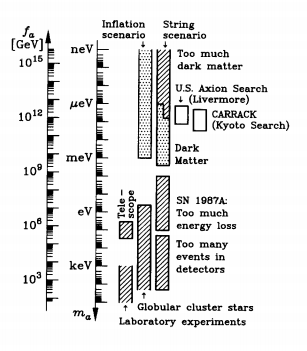
\includegraphics[width=0.6\textwidth]{1dexclusionlimit}
\caption{Constraints on the axion mass (and thus energy scale) from \cite{raffelt80}. Striped lines are constraints; blank are projected constraints; and dotted are dependent on the cosmological history of the axion.}
\end{figure}

\begin{figure}
\centering
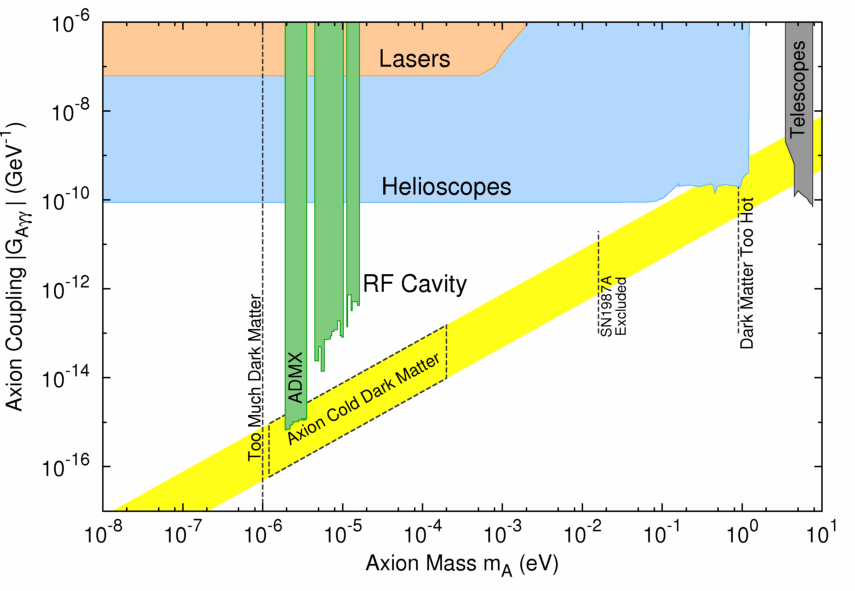
\includegraphics[width=\textwidth]{2dexclusionplot}
\caption{Summary of the ALP and axion parameter space. In yellow are shown the axion model bounds. ADMX, in green, and their experimental limits begin to constrain the axion models. Helioscopes, led by CAST, and their limits are shown in blue; photon regeneration expts labeled as Lasers exclude the upper right region but do not assume anything about dark matter so are more rigorous. The dashed line labeled SN1987A is the exclusion on the axion mass extrapolated from the observation of neutrino events from SN1987A.}
\end{figure}

\section{The Primakoff Effect}

We have referred to the Primakoff effect several times; this is the axion-two photon interaction that most axion experiments use and that is capitalized on in this work. To see how this occurs, we write the effective Lagrangian for the ALP to gluon coupling once more:

\begin{align*}
\mathcal{L} = \bar \theta g^2 G \tilde G = \frac{a}{f_a} g^2 G \tilde G
\end{align*}

This hides the fact that there is a triangle loop causing a Yukawa coupling between the axion and the intermediate fermion which couples to the gluons. Either this fermion is a heavy quark (as in the KSVZ) model, or an ordinary fermion.

The gluons can create quark-anti-quark pairs, with the pion being the lightest example. One can think of this axion-pion mixing as the effect that generates the axion mass. The pions can then decay into two photons via the Primakoff effect, which itself has a triangle loop anomaly, and this is how the axion interacts with two photons.

\section{How axions are produced as dark matter}

So far we have explained how axions in particular can be produced as the result of a new symmetry having an anomaly with QCD. Now let us consider what happens during the evolution of the axion. The potential that the axion feels is a function both of $\theta$ and T, the temperature. 

\begin{figure}
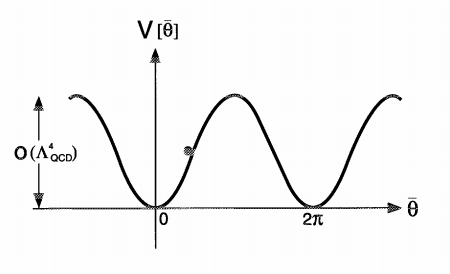
\includegraphics[width=0.6\textwidth]{vthetavstheta}
\end{figure}


\begin{figure}
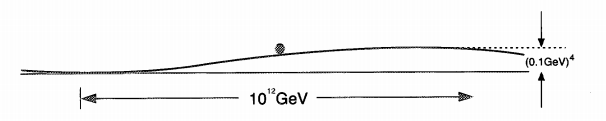
\includegraphics[width=0.6\textwidth]{axionpotential}
\caption{From \cite{kim95}; shows how slight the axion potential is.}
\end{figure}

Imagine this potential being stretched out in space, as is happening through the expansion of the universe. When the expansion slows down sufficiently so that $H \sim m_a$, the axion begins to oscillate. Because the lifetime of the axion is longer than the age of the universe, the oscillations do not die out, but the amplitude of the oscillations is decreased by the expansion of the universe. Discussion taken from Kim's "Axionic Extensions of the Standard Model".

\section{Supernova Limit}

We make a note here about the supernova limit and how it was achieved. The limit is $6 \times 10^{-11}$ 1/GeV; better than the limits produced by this experiment. However, we appeal to systematic uncertainties in the understanding of supernova physics.

\subsection{Why microwave cavities?}
The work in this thesis describes a search for dark matter axion-like particles, using a cryogenically cooled microwave cavity in a strong magnetic field. Methods to search for these dark matter particles have been ongoing for the last four decades; however, since dark matter candidates by definition interact very feebly with ordinary matter, searching for any of these particles is experimentally challenging.  As this thesis is concerned with a dark matter axion search, I will briefly review the techniques



While I will go into more detail about each of the candidates later, axions in particular also solve a problem in particle physics related to symmetry violations. 




At this point, it is firmly established that a large portion of the matter in the universe is non-luminous. Through astrophysical observations, we can estimate that the mass to light ratio in spiral galaxies is much higher than we would expect from the amount of luminous matter alone [NEEDSREF]. The existence of this gravitationally interacting matter influences the rate of structure formation in the early universe, and measurements of the cosmic microwave background can state that the observations are consistent with a $\Lambda$CDM model; that is, a model of the universe as composed of non-baryonic, non-relativistic matter [NEEDSREF]. We know very little more about this dark matter other than the conclusions stated above.

At the same time, the nature of physics at high energy (> TeV) scales is unknown. The equations that make up the Standard Model do not extend into this energy range, and current experiments that can produce physics at high energies (the LHC, other colliders) will be limited by the size of the experiments to explore energies of at most 10 TeV. Ther are many theories of physics at high energy scales; all of these predict new particles at higher energies, or additional symmetries. The high-energy particles or new effects at high energies can enter as small corrections in loop diagrams, leading to small corrections in low-energy observables. The electric dipole moment is one such observable that can be measured in laboratories but whose value is sensitive to high energy physics. The most recent measurement of the electric dipole moment of the electron \cite{acme14} done by the ACME experiment has seen a result consistent with zero, ruling out parameters of 100 TeV theories such as Supersymmetric models. These Supersymmetric (SUSY) theories are high energy theories that solve problems in high energy particle physics, and also predict a stable particle that is a very good candidate for the particle of cold dark matter.

Another probe of this high energy physics is to look for extremely light, feebly interacting particles. These particles arise as the low-mass boson accompanying the breaking of new symmetries at high energies (usually >$10^{14}$ eV). These particles, known generally as Weakly Interacting Sub-eV Particles (WISPs), are good cold dark matter candidates as well, granted that their abundance can be accounted to match the present abundance of dark matter. A particular particle belonging to the WISP category, are axion-like particles (ALPs). This denotes pseudoscalar spin 0 bosons with a non-zero coupling to two photons. ALPs take their name from the axion, a particle with the properties described above which arises from a new symmetry which was postulated by Peccei and Quinn \cite{peccei77} to solve the problem of charge and parity conservation in the theory of strong interactions when a priori there is no physical reason this CP conservation should hold.

As direct detection searches for  the SUSY dark matter candidate with no results, there is an intrinsic neutrino background that will soon limit the experiments' sensitivity within another few orders of magnitude from where they can presently search. In addition, no particles have been seen at the LHC, which expected to find new particles that would be SUSY particles. The EDM experiments have constrained different SUSY models with no observation of the electric dipole moment. At this time, it seems necessary to build small tabletop experiments that can look for other dark matter candidates, such as axion-like particles. There is a wide space in which to search for these WISPs, and having measurements allows us to constrain models. A discovery would give us clues as to the nature of physics at high energy scales, and tell us about the composition of dark matter.

\subsection{The State of Dark Matter Searches}

Starting from the assumption that dark matter is a particle, people look for heavy, stable, neutral particles, known by the acronym Weakly Interacting Massive Particles (WIMPs), under which the SUSY candidate falls. People also look for the WISPs. There are direct and indirect detection searches going on for both candidates. For WIMPS, direct searches look for WIMP to strike a nucleus, causing it to recoil. The indirect searches assume that WIMPs annihilate with each other, being their own antiparticle, and look for signatures of these events in the galaxy.

For WISPs, direct searches primarily use the ALP to two photon vertex, as it is easy to produce large electromagnetic fields in the laboratory and easy to detect photons. Searches assuming that the ALP is the dark matter are only using microwave cavities as resonant detectors \cite{admx10} although a Rydberg atom detection experiment was performed \cite{yamamoto00}. These experiments depend on the dark matter density at Earth. There are also new ideas involving the axion as inducing an oscillating electron dipole moment in nucleons \cite{budker13}, which will be sensitive to  ALPs of a different mass than those in the microwave cavity experiments. There are other experiments looking for axion-like particles, although they do not use dark matter as the source of the WISPs. These involve looking for axions produced in the sun (CAST) \cite{cast11} or directly producing axions from the two photon vertex using a laser and strong magnetic field (ALPS-I, ALPS-II) \cite{ehret10}. The direct production or light-shining-through-wall experiments has the least number of assumptions, but these experiments (solar, microwave cavity, lsw) together form a complementary way of searching for ALPs with the two-photon vertex.

There are also astrophysical arguments that can limit the coupling of the axion to the two photon vertex. The ALP, produced by various processes in red giants, neutron stars, and white dwarfs, would radiate energy from the star, altering the stellar evolution and thus stellar lifetime \cite{turner89}. By observing stellar lifetime consistent with 10$\%$, constraints on the axion coupling can be derived\cite{raffelt95}. A strong limit comes from the observation of neutrinos from the supernova explosion of SN1987A. The observation of neutrinos number and duration consistent with expectations limits the role of axions in acting as a energy loss channel. The limit is on the axion to nucelon coupling, but can be related to the axion to two photon coupling.

This dissertation will focus on a direct search for dark matter axions using microwave cavities as resonant detectors over the frequency range 33.9 to 34.5 GHz.

\subsection{Outline}

This dissertation will describe the pilot run of the Yale Microwave Cavity Experiment (YMCE) to look for dark matter ALPs in the mass range 140.2-142.7 $\mu$eV. The run set limits on the ALP-two photon coupling with sensitivity slightly better than the best previous limit set by CAST. The experiment used a microwave cavity that was tuned, immersed in a strong magnetic field - over the cavity bandwidth we would be sensitive to photons whose energy is equal to the incoming dark matter axion energy.  From the data taken, the analysis excludes axion-like particles with two-photon coupling $g_{a\gamma\gamma} < 8.6$ $1/GeV$. We end by suggesting future directions for the experiment.
The outline of the dissertation will be as follows:

\textbf{Chapter 2: Dark Matter ALPs} describes the mechanism by which these light ALPs can have the relic abundance today to match dark matter abundances observed, as well as briefly describing the specific symmetry breaking mechanism by which the axion comes about to solve the strong CP problem.

\textbf{Chapter 3: Parameter Space} goes over the current bounds on axion coupling and mass, and where microwave cavity searches fit into this field.

\textbf{Chapter 4: Detection Technique} Explains the sensitivity we can achieve using microwave cavities in strong magnetic fields, and how the expression for signal power determines what we optimize in the experiment

\textbf{Chapter 5: YMCE Experiment} goes through the components of the experiment, design of the microwave cavity, and construction of the receiver. We also go through the data taking process and summary of data taken.

\textbf{Chapter 6: Thermal Noise} The background for the experiment comes from thermal noise; we describe the expected background.

\textbf{Chapter 7: Data Analysis} puts down the analysis chain that takes the raw time domain voltage measurements and turns them into average power spectra. 

\textbf{Chapter 8: Axion Signals} We return to the expected axion power expression and walk through how that is modified when the axion energy is off resonance from the cavity resonance, but still within the cavity bandpass.

\textbf{Chapter 9:  Limits} We describe the fits and cuts applied to look for excesses in single bins that would be a hint of axion photon conversion.

\textbf{Chapter 10: Results} We present the upper bound on the ALP to two photon coupling for the mass range investigated.

\textbf{Chapter 11: Future Work} we conclude by an outlook for future work on YMCE.

\bibliographystyle{plain}
\bibliography{thesisbib}
\end{document}